\chapter{Background modeling}
\label{ch:bkgModel}

%%%%%%%%%%%%%%%%%%%%%%%%%%%%%%%%%%%%%%%%%%%%%%%%%%%%%%%%%%%%%%%%%%%%%%%%%
\section{W+jets background estimate with alpha method}

%%%%%%%%%
 \subsection{Description}
 
 %%%%%%%%%
 \subsection{Extraction of the W+jets normalization}
 
 \begin{figure}[htbp]
\centering
\includegraphics[width=0.325\textwidth]{\chnine/WVanalysis/BackgroundEstimate/HP_mj_fitting/mu/_TTbar_xwwtreeEDBR_TTBARpowheg_xww_2Gaus_ErfExp_with_pull.pdf}
\includegraphics[width=0.325\textwidth]{\chnine/WVanalysis/BackgroundEstimate/HP_mj_fitting/mu/_VV_xwwtreeEDBR_VV_xww_2_2Gaus_with_pull.pdf}
\includegraphics[width=0.325\textwidth]{\chnine/WVanalysis/BackgroundEstimate/HP_mj_fitting/mu/_STop_xwwtreeEDBR_SingleTop_xww_ExpGaus_with_pull.pdf}\\
\includegraphics[width=0.325\textwidth]{\chnine/WVanalysis/BackgroundEstimate/LP_mj_fitting/mu/_TTbar_xwwtreeEDBR_TTBARpowheg_xww_ExpGaus_with_pull.pdf}
\includegraphics[width=0.325\textwidth]{\chnine/WVanalysis/BackgroundEstimate/LP_mj_fitting/mu/_VV_xwwtreeEDBR_VV_xww_ExpGaus_with_pull.pdf}
\includegraphics[width=0.325\textwidth]{\chnine/WVanalysis/BackgroundEstimate/LP_mj_fitting/mu/_STop_xwwtreeEDBR_SingleTop_xww_ExpGaus_with_pull.pdf}\\
\caption{MC fits of non-dominant background \mJ spectra: on top (bottom) high purity (low purity) categories for the muon
channel. Left to right are the \ttbar, diboson (WW/WZ/ZZ) and Single Top processes.}
\label{fig:mcfitsjetmass_1}
\end{figure}

\begin{figure}[htbp]
\centering
\includegraphics[width=0.48\textwidth]{\chnine/WVanalysis/BackgroundEstimate/HP_mj_fitting/mu/_WJets0_xwwtreeEDBR_WJets_xww_User1_with_pull.pdf}
\includegraphics[width=0.48\textwidth]{\chnine/WVanalysis/BackgroundEstimate/LP_mj_fitting/mu/_WJets0_xwwtreeEDBR_WJets_xww_User1_with_pull.pdf}\\
\caption{MC fits of dominant W+jets background \mJ spectra: high purity (left) and low purity (right) category for the muon channel.}
\label{fig:mcfitsjetmass_1b}
\end{figure}

\begin{figure}[htbp]
\centering
\includegraphics[width=0.325\textwidth]{\chnine/WVanalysis/BackgroundEstimate/HP_mj_fitting/el/_TTbar_xwwtreeEDBR_TTBARpowheg_xww_2Gaus_ErfExp_with_pull.pdf}
\includegraphics[width=0.325\textwidth]{\chnine/WVanalysis/BackgroundEstimate/HP_mj_fitting/el/_VV_xwwtreeEDBR_VV_xww_2_2Gaus_with_pull.pdf}
\includegraphics[width=0.325\textwidth]{\chnine/WVanalysis/BackgroundEstimate/HP_mj_fitting/el/_STop_xwwtreeEDBR_SingleTop_xww_ExpGaus_with_pull.pdf}\\
\includegraphics[width=0.325\textwidth]{\chnine/WVanalysis/BackgroundEstimate/LP_mj_fitting/el/_TTbar_xwwtreeEDBR_TTBARpowheg_xww_ExpGaus_with_pull.pdf}
\includegraphics[width=0.325\textwidth]{\chnine/WVanalysis/BackgroundEstimate/LP_mj_fitting/el/_VV_xwwtreeEDBR_VV_xww_ExpGaus_with_pull.pdf}
\includegraphics[width=0.325\textwidth]{\chnine/WVanalysis/BackgroundEstimate/LP_mj_fitting/el/_STop_xwwtreeEDBR_SingleTop_xww_ExpGaus_with_pull.pdf}\\
\caption{MC fits of non-dominant background \mJ spectra: on top (bottom) high purity (low purity) categories for the electron
channel. Left to right are the \ttbar, diboson (WW/WZ/ZZ) and Single Top processes.}
\label{fig:mcfitsjetmass_2}
\end{figure}

\begin{figure}[htbp]
\centering
\includegraphics[width=0.48\textwidth]{\chnine/WVanalysis/BackgroundEstimate/HP_mj_fitting/el/_WJets0_xwwtreeEDBR_WJets_xww_User1_with_pull.pdf}
\includegraphics[width=0.48\textwidth]{\chnine/WVanalysis/BackgroundEstimate/LP_mj_fitting/el/_WJets0_xwwtreeEDBR_WJets_xww_User1_with_pull.pdf}\\
\caption{MC fits of dominant W+jets background \mJ spectra: high purity (left) and low purity (right) category for the electron channel.}
\label{fig:mcfitsjetmass_2b}
\end{figure}

\begin{figure}[htbp]
\centering
\includegraphics[width=0.48\textwidth]{\chnine/WVanalysis/BackgroundEstimate/HP_mj_fitting/mu/m_j_sideband_WJets0_xww__with_pull.pdf}
\includegraphics[width=0.48\textwidth]{\chnine/WVanalysis/BackgroundEstimate/LP_mj_fitting/mu/m_j_sideband_WJets0_xww__with_pull.pdf}\\
\includegraphics[width=0.48\textwidth]{\chnine/WVanalysis/BackgroundEstimate/HP_mj_fitting/el/m_j_sideband_WJets0_xww__with_pull.pdf}
\includegraphics[width=0.48\textwidth]{\chnine/WVanalysis/BackgroundEstimate/LP_mj_fitting/el/m_j_sideband_WJets0_xww__with_pull.pdf}\\
\caption{Fits to extract the relative shape and normalization of the W+jets contribution from
the data in the jet mass distribution. Top line fits for the muon channel: high purity (left) and low purity (right) category. Bottom line fits for
the electron channel: high purity (left) and low purity (right) category. The hashed area denotes the fit uncertainty, the shaded area the blinded W/Z/H signal region, and the vertical dashed lines separate the W, Z and H window from left to right.}
\label{fig:mjFits_data}
\end{figure}

 %%%%%%%%%
 \subsection{Extraction of the W+jets shape}
 
 %%%%%%%%%%%%%%%%%%%%%%%
%sb lo muon
%%%%%%%%%%%%%%%%%%%%%%%

\begin{figure}[htbp]
\centering
\includegraphics[width=0.325\textwidth]{\chnine/WVanalysis/BackgroundEstimate/HPW_mlvj_fitting/mu/treeEDBR_TTBARpowheg_xww_m_lvj_sb_loExp_with_pull.pdf}
\includegraphics[width=0.325\textwidth]{\chnine/WVanalysis/BackgroundEstimate/HPW_mlvj_fitting/mu/treeEDBR_VV_xww_m_lvj_sb_loExp_with_pull_log.pdf}
\includegraphics[width=0.325\textwidth]{\chnine/WVanalysis/BackgroundEstimate/HPW_mlvj_fitting/mu/treeEDBR_WJets_xww_m_lvj_sb_loExpN_with_pull_log.pdf}\\
\includegraphics[width=0.325\textwidth]{\chnine/WVanalysis/BackgroundEstimate/LPW_mlvj_fitting/mu/treeEDBR_TTBARpowheg_xww_m_lvj_sb_loExp_with_pull.pdf}
\includegraphics[width=0.325\textwidth]{\chnine/WVanalysis/BackgroundEstimate/LPW_mlvj_fitting/mu/treeEDBR_VV_xww_m_lvj_sb_loExp_with_pull_log.pdf}
\includegraphics[width=0.325\textwidth]{\chnine/WVanalysis/BackgroundEstimate/LPW_mlvj_fitting/mu/treeEDBR_WJets_xww_m_lvj_sb_loExpN_with_pull_log.pdf}\\
\caption{MC fits of non-dominant background $m_{\ell\nu j}$ spectra in the \mJ sideband: on top (bottom) high purity (low purity) categories
for the muon channel. Left to right are the \ttbar, diboson (WW/WZ/ZZ) and Single Top processes.}
\label{fig:sbfitmlvj_1}
\end{figure}

\begin{figure}[htbp]
\centering
\includegraphics[width=0.48\textwidth]{\chnine/WVanalysis/BackgroundEstimate/HPW_mlvj_fitting/mu/treeEDBR_WJets_xww_m_lvj_sb_loExpN_with_pull_log.pdf}
\includegraphics[width=0.48\textwidth]{\chnine/WVanalysis/BackgroundEstimate/LPW_mlvj_fitting/mu/treeEDBR_WJets_xww_m_lvj_sb_loExpN_with_pull_log.pdf}\\
\caption{MC fits of dominant W+jets background $m_{\ell\nu j}$ spectra in the \mJ sideband:
high purity (left) and low purity (right) category for the muon channel.}
\label{fig:sbfitmlvj_1b}
\end{figure}

%%%%%%%%%%%%%%%%%%%%%%%
%sb lo electron
%%%%%%%%%%%%%%%%%%%%%%%

\begin{figure}[htbp]
\centering
\includegraphics[width=0.325\textwidth]{\chnine/WVanalysis/BackgroundEstimate/HPW_mlvj_fitting/el/treeEDBR_TTBARpowheg_xww_m_lvj_sb_loExp_with_pull.pdf}
\includegraphics[width=0.325\textwidth]{\chnine/WVanalysis/BackgroundEstimate/HPW_mlvj_fitting/el/treeEDBR_VV_xww_m_lvj_sb_loExp_with_pull_log.pdf}
\includegraphics[width=0.325\textwidth]{\chnine/WVanalysis/BackgroundEstimate/HPW_mlvj_fitting/el/treeEDBR_WJets_xww_m_lvj_sb_loExpN_with_pull_log.pdf}\\
\includegraphics[width=0.325\textwidth]{\chnine/WVanalysis/BackgroundEstimate/LPW_mlvj_fitting/el/treeEDBR_TTBARpowheg_xww_m_lvj_sb_loExp_with_pull.pdf}
\includegraphics[width=0.325\textwidth]{\chnine/WVanalysis/BackgroundEstimate/LPW_mlvj_fitting/el/treeEDBR_VV_xww_m_lvj_sb_loExp_with_pull_log.pdf}
\includegraphics[width=0.325\textwidth]{\chnine/WVanalysis/BackgroundEstimate/LPW_mlvj_fitting/el/treeEDBR_WJets_xww_m_lvj_sb_loExpN_with_pull_log.pdf}\\
\caption{MC fits of non-dominant background $m_{\ell\nu j}$ spectra in the \mJ sideband: on top (bottom) high purity (low purity) categories
for the electron channel. Left to right are the \ttbar, diboson (WW/WZ/ZZ) and Single Top processes.}
\label{fig:sbfitmlvj_2}
\end{figure}

\begin{figure}[htbp]
\centering
\includegraphics[width=0.48\textwidth]{\chnine/WVanalysis/BackgroundEstimate/HPW_mlvj_fitting/el/treeEDBR_WJets_xww_m_lvj_sb_loExpN_with_pull_log.pdf}
\includegraphics[width=0.48\textwidth]{\chnine/WVanalysis/BackgroundEstimate/LPW_mlvj_fitting/el/treeEDBR_WJets_xww_m_lvj_sb_loExpN_with_pull_log.pdf}\\
\caption{MC fits of dominant W+jets background $m_{\ell\nu j}$ spectra in the \mJ sideband:
high purity (left) and low purity (right) category for the electron channel.}
\label{fig:sbfitmlvj_2b}
\end{figure}

%%%%%%%%%%%%%%%%%%%%%%%
%MWV fits in sb lo with data
%%%%%%%%%%%%%%%%%%%%%%%

\begin{figure}[htbp]
\centering
\includegraphics[width=0.48\textwidth]{\chnine/WVanalysis/BackgroundEstimate/HPW_mlvj_fitting/mu/m_lvj_sb_lo_WJets0_xww__with_pull_log.pdf}
\includegraphics[width=0.48\textwidth]{\chnine/WVanalysis/BackgroundEstimate/LPW_mlvj_fitting/mu/m_lvj_sb_lo_WJets0_xww__with_pull_log.pdf}\\
\includegraphics[width=0.48\textwidth]{\chnine/WVanalysis/BackgroundEstimate/HPW_mlvj_fitting/el/m_lvj_sb_lo_WJets0_xww__with_pull_log.pdf}
\includegraphics[width=0.48\textwidth]{\chnine/WVanalysis/BackgroundEstimate/LPW_mlvj_fitting/el/m_lvj_sb_lo_WJets0_xww__with_pull_log.pdf}\\
\caption{The fits for $F_{data,LSB}(m_{\ell\nu j})$ for both electron (bottom) and muon (top) channels, high purity (left) and low purity (right) categories.}
\label{fig:sbfitmlvj_data}
\end{figure}

%%%%%%%%%%%%%%%%%%%%%%%
%WW signal region muon
%%%%%%%%%%%%%%%%%%%%%%%

\begin{figure}[htbp]
\centering
\includegraphics[width=0.325\textwidth]{\chnine/WVanalysis/BackgroundEstimate/HPW_mlvj_fitting/mu/treeEDBR_TTBARpowheg_xww_m_lvj_signal_regionExp_with_pull_log.pdf}
\includegraphics[width=0.325\textwidth]{\chnine/WVanalysis/BackgroundEstimate/HPW_mlvj_fitting/mu/treeEDBR_VV_xww_m_lvj_signal_regionExpN_with_pull_log.pdf}
\includegraphics[width=0.325\textwidth]{\chnine/WVanalysis/BackgroundEstimate/HPW_mlvj_fitting/mu/treeEDBR_WJets_xww_m_lvj_signal_regionExpN_with_pull_log.pdf}\\
\includegraphics[width=0.325\textwidth]{\chnine/WVanalysis/BackgroundEstimate/LPW_mlvj_fitting/mu/treeEDBR_TTBARpowheg_xww_m_lvj_signal_regionExp_with_pull_log.pdf}
\includegraphics[width=0.325\textwidth]{\chnine/WVanalysis/BackgroundEstimate/LPW_mlvj_fitting/mu/treeEDBR_VV_xww_m_lvj_signal_regionExpN_with_pull_log.pdf}
\includegraphics[width=0.325\textwidth]{\chnine/WVanalysis/BackgroundEstimate/LPW_mlvj_fitting/mu/treeEDBR_WJets_xww_m_lvj_signal_regionExpN_with_pull_log.pdf}\\
\caption{MC fits of non-dominant background $m_{\ell\nu j}$ spectra in the \mJ signal region for events in the WW category: on top (bottom) high purity (low purity) categories for the muon channel. Left to right are the \ttbar, diboson (WW/WZ/ZZ) and Single Top processes.}
\label{fig:srWfitmlvj_1}
\end{figure}

\begin{figure}[htbp]
\centering
\includegraphics[width=0.48\textwidth]{\chnine/WVanalysis/BackgroundEstimate/HPW_mlvj_fitting/mu/treeEDBR_WJets_xww_m_lvj_signal_regionExpN_with_pull_log.pdf}
\includegraphics[width=0.48\textwidth]{\chnine/WVanalysis/BackgroundEstimate/LPW_mlvj_fitting/mu/treeEDBR_WJets_xww_m_lvj_signal_regionExpN_with_pull_log.pdf}\\
\caption{MC fits of dominant W+jets background $m_{\ell\nu j}$ spectra in the \mJ signal region for events in the WW category:
high purity (left) and low purity (right) category for the muon channel.}
\label{fig:srWfitmlvj_1b}
\end{figure}

%%%%%%%%%%%%%%%%%%%%%%%
%WW signal region electron
%%%%%%%%%%%%%%%%%%%%

\begin{figure}[htbp]
\centering
\includegraphics[width=0.325\textwidth]{\chnine/WVanalysis/BackgroundEstimate/HPW_mlvj_fitting/el/treeEDBR_TTBARpowheg_xww_m_lvj_signal_regionExp_with_pull_log.pdf}
\includegraphics[width=0.325\textwidth]{\chnine/WVanalysis/BackgroundEstimate/HPW_mlvj_fitting/el/treeEDBR_VV_xww_m_lvj_signal_regionExpN_with_pull_log.pdf}
\includegraphics[width=0.325\textwidth]{\chnine/WVanalysis/BackgroundEstimate/HPW_mlvj_fitting/el/treeEDBR_WJets_xww_m_lvj_signal_regionExpN_with_pull_log.pdf}\\
\includegraphics[width=0.325\textwidth]{\chnine/WVanalysis/BackgroundEstimate/LPW_mlvj_fitting/el/treeEDBR_TTBARpowheg_xww_m_lvj_signal_regionExp_with_pull_log.pdf}
\includegraphics[width=0.325\textwidth]{\chnine/WVanalysis/BackgroundEstimate/LPW_mlvj_fitting/el/treeEDBR_VV_xww_m_lvj_signal_regionExpN_with_pull_log.pdf}
\includegraphics[width=0.325\textwidth]{\chnine/WVanalysis/BackgroundEstimate/LPW_mlvj_fitting/el/treeEDBR_WJets_xww_m_lvj_signal_regionExpN_with_pull_log.pdf}\\
\caption{MC fits of non-dominant background $m_{\ell\nu j}$ spectra in the \mJ signal region for events in the WW category: on top (bottom) high purity (low purity) categories for the electron channel. Left to right are the \ttbar, diboson (WW/WZ/ZZ) and Single Top processes.}
\label{fig:srWfitmlvj_2}
\end{figure}

\begin{figure}[htbp]
\centering
\includegraphics[width=0.48\textwidth]{\chnine/WVanalysis/BackgroundEstimate/HPW_mlvj_fitting/el/treeEDBR_WJets_xww_m_lvj_signal_regionExpN_with_pull_log.pdf}
\includegraphics[width=0.48\textwidth]{\chnine/WVanalysis/BackgroundEstimate/LPW_mlvj_fitting/el/treeEDBR_WJets_xww_m_lvj_signal_regionExpN_with_pull_log.pdf}\\
\caption{MC fits of dominant W+jets background $m_{\ell\nu j}$ spectra in the \mJ signal region for events in the WW category:
high purity (left) and low purity (right) category for the electron channel.}
\label{fig:srWfitmlvj_2b}
\end{figure}

%%%%%%%%%%%%%%%%%%%%%%%
%WZ signal reion muon
%%%%%%%%%%%%%%%%%%%%%%%

\begin{figure}[htbp]
\centering
\includegraphics[width=0.325\textwidth]{\chnine/WVanalysis/BackgroundEstimate/HPZ_mlvj_fitting/mu/treeEDBR_TTBARpowheg_xww_m_lvj_signal_regionExp_with_pull_log.pdf}
\includegraphics[width=0.325\textwidth]{\chnine/WVanalysis/BackgroundEstimate/HPZ_mlvj_fitting/mu/treeEDBR_VV_xww_m_lvj_signal_regionExpN_with_pull_log.pdf}
\includegraphics[width=0.325\textwidth]{\chnine/WVanalysis/BackgroundEstimate/HPZ_mlvj_fitting/mu/treeEDBR_WJets_xww_m_lvj_signal_regionExpN_with_pull_log.pdf}\\
\includegraphics[width=0.325\textwidth]{\chnine/WVanalysis/BackgroundEstimate/LPZ_mlvj_fitting/mu/treeEDBR_TTBARpowheg_xww_m_lvj_signal_regionExp_with_pull_log.pdf}
\includegraphics[width=0.325\textwidth]{\chnine/WVanalysis/BackgroundEstimate/LPZ_mlvj_fitting/mu/treeEDBR_VV_xww_m_lvj_signal_regionExpN_with_pull_log.pdf}
\includegraphics[width=0.325\textwidth]{\chnine/WVanalysis/BackgroundEstimate/LPZ_mlvj_fitting/mu/treeEDBR_WJets_xww_m_lvj_signal_regionExpN_with_pull_log.pdf}\\
\caption{MC fits of non-dominant background $m_{\ell\nu j}$ spectra in the \mJ signal region for events in the WZ category: on top (bottom) high purity (low purity) categories for the muon channel. Left to right are the \ttbar, diboson (WW/WZ/ZZ) and Single Top processes.}
\label{fig:srZfitmlvj_1}
\end{figure}

\begin{figure}[htbp]
\centering
\includegraphics[width=0.48\textwidth]{\chnine/WVanalysis/BackgroundEstimate/HPZ_mlvj_fitting/mu/treeEDBR_WJets_xww_m_lvj_signal_regionExpN_with_pull_log.pdf}
\includegraphics[width=0.48\textwidth]{\chnine/WVanalysis/BackgroundEstimate/LPZ_mlvj_fitting/mu/treeEDBR_WJets_xww_m_lvj_signal_regionExpN_with_pull_log.pdf}\\
\caption{MC fits of dominant W+jets background $m_{\ell\nu j}$ spectra in the \mJ signal region for events in the WZ category:
high purity (left) and low purity (right) category for the muon channel.}
\label{fig:srZfitmlvj_1b}
\end{figure}

%%%%%%%%%%%%%%%%%%%%%%%
%WZ signal reion electron
%%%%%%%%%%%%%%%%%%%%%%%

\begin{figure}[htbp]
\centering
\includegraphics[width=0.325\textwidth]{\chnine/WVanalysis/BackgroundEstimate/HPZ_mlvj_fitting/el/treeEDBR_TTBARpowheg_xww_m_lvj_signal_regionExp_with_pull_log.pdf}
\includegraphics[width=0.325\textwidth]{\chnine/WVanalysis/BackgroundEstimate/HPZ_mlvj_fitting/el/treeEDBR_VV_xww_m_lvj_signal_regionExpN_with_pull_log.pdf}
\includegraphics[width=0.325\textwidth]{\chnine/WVanalysis/BackgroundEstimate/HPZ_mlvj_fitting/el/treeEDBR_WJets_xww_m_lvj_signal_regionExpN_with_pull_log.pdf}\\
\includegraphics[width=0.325\textwidth]{\chnine/WVanalysis/BackgroundEstimate/LPZ_mlvj_fitting/el/treeEDBR_TTBARpowheg_xww_m_lvj_signal_regionExp_with_pull_log.pdf}
\includegraphics[width=0.325\textwidth]{\chnine/WVanalysis/BackgroundEstimate/LPZ_mlvj_fitting/el/treeEDBR_VV_xww_m_lvj_signal_regionExpN_with_pull_log.pdf}
\includegraphics[width=0.325\textwidth]{\chnine/WVanalysis/BackgroundEstimate/LPZ_mlvj_fitting/el/treeEDBR_WJets_xww_m_lvj_signal_regionExpN_with_pull_log.pdf}\\
\caption{MC fits of non-dominant background $m_{\ell\nu j}$ spectra in the \mJ signal region for events in the WZ category: on top (bottom) high purity (low purity) categories for the electron channel. Left to right are the \ttbar, diboson (WW/WZ/ZZ) and Single Top processes.}
\label{fig:srZfitmlvj_2}
\end{figure}

\begin{figure}[htbp]
\centering
\includegraphics[width=0.48\textwidth]{\chnine/WVanalysis/BackgroundEstimate/HPZ_mlvj_fitting/el/treeEDBR_WJets_xww_m_lvj_signal_regionExpN_with_pull_log.pdf}
\includegraphics[width=0.48\textwidth]{\chnine/WVanalysis/BackgroundEstimate/LPZ_mlvj_fitting/el/treeEDBR_WJets_xww_m_lvj_signal_regionExpN_with_pull_log.pdf}\\
\caption{MC fits of dominant W+jets background $m_{\ell\nu j}$ spectra in the \mJ signal region for events in the WZ category:
high purity (left) and low purity (right) category for the electron channel.}
\label{fig:srZfitmlvj_2b}
\end{figure}

%%%%%%%%%%%%%%%%%%%%%%%
%correction for WW signal region
%%%%%%%%%%%%%%%%%%%%%%%

\begin{figure}[htbp]
\centering
\includegraphics[width=0.48\textwidth]{\chnine/WVanalysis/BackgroundEstimate/HPW_mlvj_fitting/mu/correction_pdf_WJets0_xww_ExpN_M_lvj_signal_region_to_sideband.png}
\includegraphics[width=0.48\textwidth]{\chnine/WVanalysis/BackgroundEstimate/HPZ_mlvj_fitting/mu/correction_pdf_WJets0_xww_ExpN_M_lvj_signal_region_to_sideband.png}\\
\includegraphics[width=0.48\textwidth]{\chnine/WVanalysis/BackgroundEstimate/LPW_mlvj_fitting/mu/correction_pdf_WJets0_xww_ExpN_M_lvj_signal_region_to_sideband.png}
\includegraphics[width=0.48\textwidth]{\chnine/WVanalysis/BackgroundEstimate/LPZ_mlvj_fitting/mu/correction_pdf_WJets0_xww_ExpN_M_lvj_signal_region_to_sideband.png}\\
\caption{The functions $\alpha_{MC}({m_{\ell\nu j}})$ for the muon high purity category (top), low purity (bottom) categories
used for extrapolate W+jets $m_{\ell\nu j}$ shape in the WW (left) and WZ (right) signal regions.}
\label{fig:alphas_VW_1}
\end{figure}

\begin{figure}[htbp]
\centering
\includegraphics[width=0.48\textwidth]{\chnine/WVanalysis/BackgroundEstimate/HPW_mlvj_fitting/el/correction_pdf_WJets0_xww_ExpN_M_lvj_signal_region_to_sideband.png}
\includegraphics[width=0.48\textwidth]{\chnine/WVanalysis/BackgroundEstimate/HPZ_mlvj_fitting/el/correction_pdf_WJets0_xww_ExpN_M_lvj_signal_region_to_sideband.png}\\
\includegraphics[width=0.48\textwidth]{\chnine/WVanalysis/BackgroundEstimate/LPW_mlvj_fitting/el/correction_pdf_WJets0_xww_ExpN_M_lvj_signal_region_to_sideband.png}
\includegraphics[width=0.48\textwidth]{\chnine/WVanalysis/BackgroundEstimate/LPZ_mlvj_fitting/el/correction_pdf_WJets0_xww_ExpN_M_lvj_signal_region_to_sideband.png}\\
\caption{The functions $\alpha_{MC}(m_{\ell\nu j})$ for the electron high purity category (top), low purity (bottom) categories
used for extrapolate W+jets $m_{\ell\nu j}$ shape in the WW (left) and WZ (right) signal regions.}
\label{fig:alphas_VW_2}
\end{figure}

%%%%%%%%%
%\subsection{Closure check of the method}

\clearpage
%%%%%%%%%%%%%%%%%%%%%%%%%%%%%%%%%%%%%%%%%%%%%%%%%%%%%%%%%%%%%%%%%%%%%%%%%
\section{Top quark production}

%%%%%%%%%
\subsection*{8 TeV analysis}

\begin{figure}[bh!p]
\centering
\begin{tabular}{lr}
\includegraphics[width=0.5\textwidth]{\chnine/WHanalysis/ttbarCP/ele/pruned-mass.pdf} &
\includegraphics[width=0.5\textwidth]{\chnine/WHanalysis/ttbarCP/mu/pruned-mass.pdf} \\
\end{tabular}
\caption{Pruned jet mass for electron channel (left) and muon channel (right) for events with
$40~<~m_{jet}^{pruned}~<~150$ GeV in the $t\bar{t}$ control sample.}
\label{fig:ttbarCP1}
\end{figure}

\begin{figure}[h!bp]
\centering
\begin{tabular}{lr}
\includegraphics[width=0.5\textwidth]{\chnine/WHanalysis/ttbarCP/ele/leptonic-top-mass.pdf} &
\includegraphics[width=0.5\textwidth]{\chnine/WHanalysis/ttbarCP/mu/leptonic-top-mass.pdf} \\
\includegraphics[width=0.5\textwidth]{\chnine/WHanalysis/ttbarCP/ele/hadronic-top-mass.pdf} &
\includegraphics[width=0.5\textwidth]{\chnine/WHanalysis/ttbarCP/mu/hadronic-top-mass.pdf} \\
\end{tabular}
\caption{$m_{top}^{leptonic}$ (top) and $m_{top}^{hadronic}$ (bottom) for electron channel (left) and muon channel (right) for events with
$40~<~m_{jet}^{pruned}~<~150$ GeV in the $t\bar{t}$ control sample.}
\label{fig:ttbarCP2}
\end{figure}

\begin{figure}[h!bp]
\centering
\begin{tabular}{lr}
\includegraphics[width=0.5\textwidth]{\chnine/WHanalysis/ttbarCP/ele/dibosons-invmass.pdf} &
\includegraphics[width=0.5\textwidth]{\chnine/WHanalysis/ttbarCP/mu/dibosons-invmass.pdf} \\
\includegraphics[width=0.5\textwidth]{\chnine/WHanalysis/ttbarCP/ele/dibosons-invmass-log.pdf} &
\includegraphics[width=0.5\textwidth]{\chnine/WHanalysis/ttbarCP/mu/dibosons-invmass-log.pdf} \\
\end{tabular}
\caption{$m_{WH}$ in linear (top) and log (bottom) scale for electron channel (left) and muon channel (right) for events with
$40~<~m_{jet}^{pruned}~<~150$ GeV in the $t\bar{t}$ control sample.}
\label{fig:ttbarCP3}
\end{figure}

\clearpage
%%%%%%%%%
\subsection*{13 TeV analysis}

 \begin{figure}[htbp]
 \centering
 \begin{tabular}{cc}
 \includegraphics[width=0.45\textwidth]{chapters/Chapter8-EventSelection/Figures/WVanalysis/ControlPlots_TTbar/mu/jet_mass_pr_0}
 \includegraphics[width=0.45\textwidth]{chapters/Chapter8-EventSelection/Figures/WVanalysis/ControlPlots_TTbar/el/jet_mass_pr_0}\\
 \includegraphics[width=0.45\textwidth]{chapters/Chapter8-EventSelection/Figures/WVanalysis/ControlPlots_TTbar/mu/jet_tau2tau1_0}
 \includegraphics[width=0.45\textwidth]{chapters/Chapter8-EventSelection/Figures/WVanalysis/ControlPlots_TTbar/el/jet_tau2tau1_0}\\
 \end{tabular}
 \caption{Comparison plots between data and MC for different observables, in the \ttbar control region.
 Top: pruned jet mass. Bottom: N-subjettiness. 
 Left: muon channel, right: electron channel. }
 \label{fig:TTbar_controlPlots_4}
 \end{figure}

 \begin{figure}[htbp]
 \centering
 \begin{tabular}{cc}
 \includegraphics[width=0.45\textwidth]{chapters/Chapter8-EventSelection/Figures/WVanalysis/ControlPlots_TTbar/mu/nPV_0}
 \includegraphics[width=0.45\textwidth]{chapters/Chapter8-EventSelection/Figures/WVanalysis/ControlPlots_TTbar/el/nPV_0}\\
 \includegraphics[width=0.45\textwidth]{chapters/Chapter8-EventSelection/Figures/WVanalysis/ControlPlots_TTbar/mu/l_pt_0}
 \includegraphics[width=0.45\textwidth]{chapters/Chapter8-EventSelection/Figures/WVanalysis/ControlPlots_TTbar/el/l_pt_0}\\
 \includegraphics[width=0.45\textwidth]{chapters/Chapter8-EventSelection/Figures/WVanalysis/ControlPlots_TTbar/mu/l_eta_0}
 \includegraphics[width=0.45\textwidth]{chapters/Chapter8-EventSelection/Figures/WVanalysis/ControlPlots_TTbar/el/l_eta_0}\\
 \end{tabular}
 \caption{Comparison plots between data and MC for different observables, in the \ttbar control region.
 From top to bottom: number of primary vertices, lepton \pt, lepton $\eta$. 
 Left: muon channel, right: electron channel. }
 \label{fig:TTbar_controlPlots_1}
 \end{figure}

 \begin{figure}[htbp]
 \centering
 \begin{tabular}{cc}
 \includegraphics[width=0.45\textwidth]{chapters/Chapter8-EventSelection/Figures/WVanalysis/ControlPlots_TTbar/mu/pfMET_0}
 \includegraphics[width=0.45\textwidth]{chapters/Chapter8-EventSelection/Figures/WVanalysis/ControlPlots_TTbar/el/pfMET_0}\\
 \includegraphics[width=0.45\textwidth]{chapters/Chapter8-EventSelection/Figures/WVanalysis/ControlPlots_TTbar/mu/v_pt_0}
 \includegraphics[width=0.45\textwidth]{chapters/Chapter8-EventSelection/Figures/WVanalysis/ControlPlots_TTbar/el/v_pt_0}\\
 \includegraphics[width=0.45\textwidth]{chapters/Chapter8-EventSelection/Figures/WVanalysis/ControlPlots_TTbar/mu/v_mt_0}
 \includegraphics[width=0.45\textwidth]{chapters/Chapter8-EventSelection/Figures/WVanalysis/ControlPlots_TTbar/el/v_mt_0}\\
 \end{tabular}
 \caption{Comparison plots between data and MC for different observables, in the \ttbar control region.
 From top to bottom: \MET, leptonic W \pt, transverse mass of the leptonic W. 
 Left: muon channel, right: electron channel. }
 \label{fig:TTbar_controlPlots_2}
 \end{figure}

 \begin{figure}[htbp]
 \centering
 \begin{tabular}{cc}
 \includegraphics[width=0.45\textwidth]{chapters/Chapter8-EventSelection/Figures/WVanalysis/ControlPlots_TTbar/mu/ungroomed_jet_pt_0}
 \includegraphics[width=0.45\textwidth]{chapters/Chapter8-EventSelection/Figures/WVanalysis/ControlPlots_TTbar/el/ungroomed_jet_pt_0}\\
 \includegraphics[width=0.45\textwidth]{chapters/Chapter8-EventSelection/Figures/WVanalysis/ControlPlots_TTbar/mu/ungroomed_jet_eta_0}
 \includegraphics[width=0.45\textwidth]{chapters/Chapter8-EventSelection/Figures/WVanalysis/ControlPlots_TTbar/el/ungroomed_jet_eta_0}\\
 \end{tabular}
 \caption{Comparison plots between data and MC for different observables, in the \ttbar control region.
 Top: \pt of the leading AK8 jet. Bottom: $\eta$ of the leading AK8 jet. 
 Left: muon channel, right: electron channel. }
 \label{fig:TTbar_controlPlots_3}
 \end{figure}
 
 \clearpage
 %%%%%%%%%%%%%%%%%%%%%%%%%%%%%%%%%%%%%%%%%%%%%%%%%%%%%%%%%%%%%%%%%%%%%%%%%
\section{Systematic uncertainties in the background estimation}
